\saltoPag%
\section{UNIDAD 2}
    \subsection{Experimentos y teorías}
        \begin{center} \textcolor{red}{\underline{Exp. De Millikan}} \end{center}
        \indent Determinación de la masa específica del electrón.
        \begin{center} 
            \begin{tabular}{|| c | c ||}
                \hline
                \textbf{Concepto}    &   \textbf{Valores}     \\
                \hline
                \hline
                Relación carga/masa  &   $-1,76 \times 10^8 C/g$ \\
                \hline
                Carga del $e^-$      &  $-1.60 \times 10^{-19} C$ \\
                \hline
                Masa del $e^-$       &  $9,10 \times 10^{-28} g$ \\
                \hline
            \end{tabular}
        \end{center}

        \begin{center} 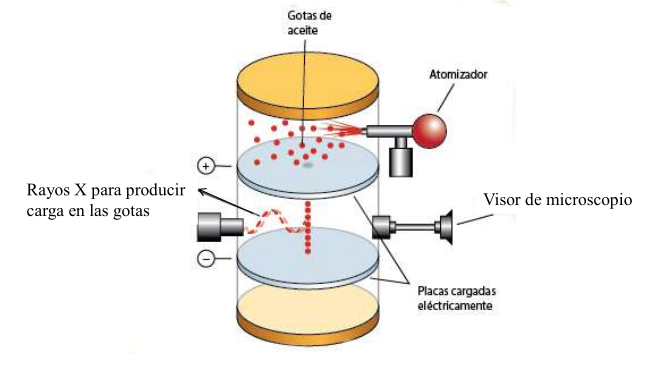
\includegraphics[width=8cm]{./imagenes/experienciaMIllikan.png} \end{center}

        \begin{center} \textcolor{red}{\underline{Radiactividad}} \end{center}
            \begin{center} 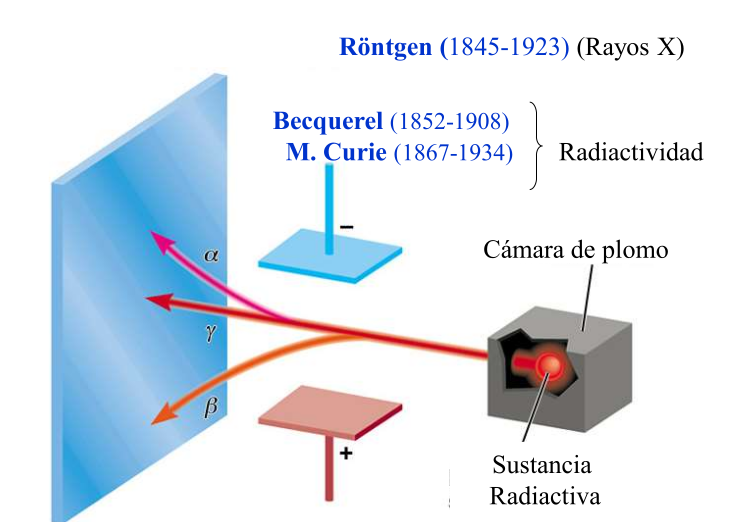
\includegraphics[width=8cm]{./imagenes/radiactividadExperimento.png} \end{center}

        \begin{center} \textcolor{red}{\underline{Modelo de Thomson}} \end{center}
            \begin{center} 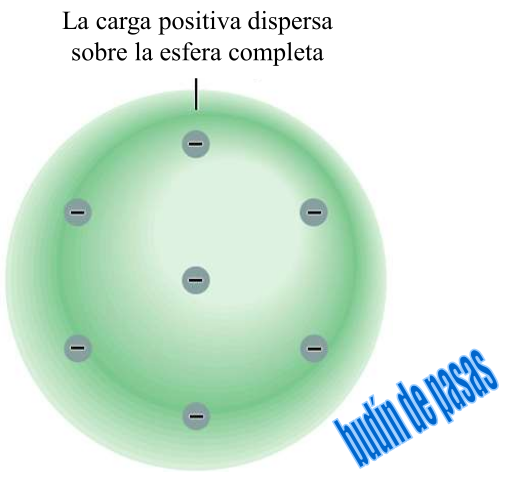
\includegraphics[width=7cm]{./imagenes/modeloDeThomson.png} \end{center}
        
        \begin{center} \textcolor{red}{\underline{Exp. De Rutherford}} \end{center}
            \begin{enumerate} 
                \item La carga positiva de un átomo está concentrada en su núcleo.
                \item El protón ($p$) tiene una carga $+$, el electrón tiene carga $-$.
                \item La masa del protón es 1840 $\times$ masa del $e^-$ ($1.67 \ times 10^{-24}g$).
            \end{enumerate}

            \begin{center} 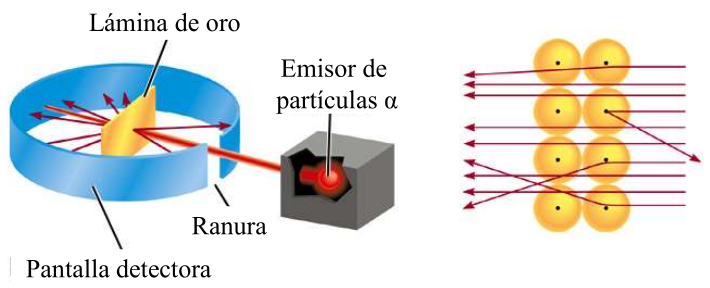
\includegraphics[width=8cm]{./imagenes/experimentoRutherford.png} \end{center}

        \begin{center} \textcolor{red}{\underline{El neutrón}} \end{center}
            \begin{center} 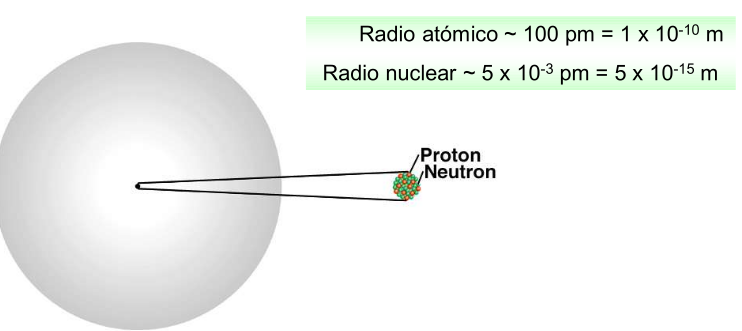
\includegraphics[width=7cm] {./imagenes/neutron.png} \end{center}

        \begin{center} \textcolor{red}{\underline{Exp. De Chadwick}} \end{center}
            \indent Se bombardeo una delgada lámina de $Be$ con partículas $\alpha$, el metal emitió una radiación de muy alta energía, similar a los rayos $\gamma$. Posteriormente se demostró que eran neutrones.

        \begin{center}
            \begin{tabular}{| c | c | c | c |}
                \hline
                \textbf{\scalebox{0.8}{Partícula}}  &
                \textbf{\scalebox{0.8}{Masa(g)}}   &
                \textbf{\scalebox{0.8}{Carga(C)}}    &
                \textbf{\scalebox{0.8}{Unidad de carga}} \\
                \hline
                \scalebox{0.8}{Electrón}            &
                \scalebox{0.8}{$9,109 \times 10^{-28}$}     &
                \scalebox{0.8}{$-1,602 \times 10^{-19}$}   & 
                \scalebox{0.8}{$-1$}    \\
                \hline
                \scalebox{0.8}{Protón} &
                \scalebox{0.8}{$1,672 \times 10^{-24}$} &
                \scalebox{0.8}{$+1,602 \times 10^{-19}$} &
                \scalebox{0.8}{$+1$} \\
                \hline
                \scalebox{0.8}{Neutrón} &
                \scalebox{0.8}{$1,674 \times 10^{-24}$} &
                \scalebox{0.8}{$0$} &
                \scalebox{0.8}{$0$} \\
                \hline
            \end{tabular}
        \end{center}

        \begin{center} \textcolor{red}{\underline{Teoría cuántica - Propiedades de las ondas}} \end{center}
            \begin{center} 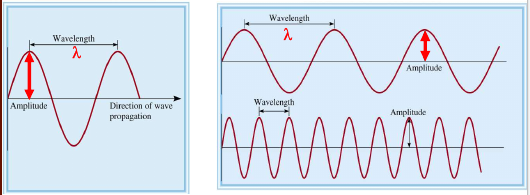
\includegraphics[width=8cm]{./imagenes/propiedadesOndas.png} \end{center}

            \begin{itemize} 
                \item \textcolor{red}{\textbf{Longitud de onda ($\lambda$):}} distancia que existe entre dos puntos idénticos en una serie de ondas.
                \item \textcolor{red}{\textbf{Amplitud:}} distancia vertical desde el punto medio de la curva hasta una cresta (punto máximo) o un valle (punto mínimo).
            \end{itemize}

        \begin{center} \textcolor{red}{\underline{Radiación electromagnética}} \end{center}
            \indent Maxwell $\rightsquigarrow$ \textit{"La luz está formada por ondas electromagnéticas"}.
            \saltoPag%
            \begin{center} 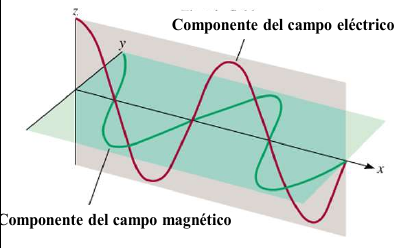
\includegraphics[width=7cm]{./imagenes/componentesDeUnaOnda.png} \end{center}
            \indent Velocidad de la luz en el vacío $\approx$ $3 \times 10^{8} m/s$.

        \begin{center} \textcolor{red}{\underline{Teoría cuántica de Planck}} \end{center}
            \indent Los sólidos cuando se calientan emiten radiación electromagnética que abarca una gama de longitudes de onda. \\
            \indent Planck definió al \textcolor{red}{\textit{cuanto}} como la mínima cantidad de energía que podía ser emitida o absorbida en forma de radiación electromagnética.

            \begin{center} \begin{tabular}{| c |} \hline \\ $E = \hbar \times v$ \\ \hline \end{tabular} \end{center}
            \indent Siendo "$\hbar$" la constante de Planck y vale $6,63 \times 10^{-34} J.s$ \\
            \indent La energía siempre se emite en múltiplos enteros y positivos de $\hbar \times v$.

    \subsection{Efecto fotoeléctrico}
        \begin{center} 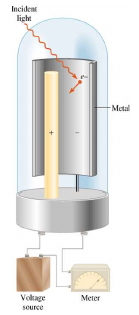
\includegraphics[width=5cm]{./imagenes/efectoFotoelectrico.png} \end{center}
        \indent La luz tiene:
        \begin{enumerate} 
            \item una naturaleza como onda electromagnética.
            \item una naturaleza como partícula (fotón).
        \end{enumerate}
        \begin{center} 
            $E = \hbar \times v$ \\
            $E = BE + KE$
        \end{center}
        \indent Siendo:
        \begin{itemize}
            \item BE\: energía de enlace.
            \item KE\: energía cinética.
        \end{itemize}
        \begin{center} \textit{Mayor frecuencia $\rightarrow$ mayor energía cinética} \end{center}
        \begin{center} \textit{Rayo de luz más intenso $\rightarrow$ mayor número de electrones emitidos.} \end{center}
        \indent La frecuencia mínima para extraer un electrón de un átomo (efecto fotoeléctrico) se denomina ''frecuencia umbral'' ($v_0$).
        \begin{center} 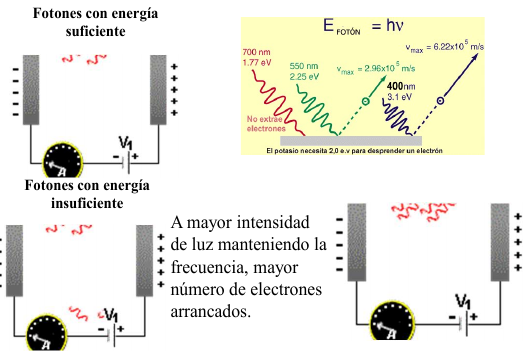
\includegraphics[width=7cm]{./imagenes/frecuenciaUmbral.png} \end{center}

    \subsection{Espectros atómicos}
        \indent Cuando a los elementos en estado gaseoso se les suministra energía (descarga eléctrica, calentamiento, etc.) éstos emiten radiaciones de determinadas longitudes de onda. \\
        \indent Estas radiaciones dispersadas en un prisma de un espectroscopio se ven como una serie de rayas, y el conjunto de las mismas es lo que se conoce como espectro de emisión. \\
        \indent Igualmente, si una luz continua atraviesa una sustancia, ésta absorbe unas determinadas radiaciones que aparecen como rayas negras en el fondo continuo (espectro de absorción). \\

    \subsection{Teoría y modelo de Bohr}
        \indent Espectro de emisión del átomo de hidrógeno.
        \begin{center} 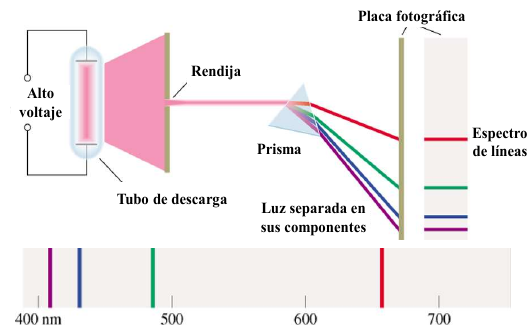
\includegraphics[width=7cm]{./imagenes/espectroEmisionHidrogeno.png} \end{center}
        \begin{enumerate}
            \item Los electrones se mueven en órbitas de energías específicas.
            \item Las energías del electrón están cuantiadas.
            \item Cuando existe una emisión de luz, los electrones se mueven de un nivel de energía mayor a otro menor emiten energía en forma de fotones.
            \saltoPag%
            \begin{center} 
                $E_N = - R_H (\frac{1}{n^2})$
            \end{center}
        \end{enumerate}
        \indent Siendo:
        \begin{itemize}
            \item $n \text{número cuántico principal} = 1,2,3 ... \text{nivel energético}$.
            \item $R_H \text{Constante de Rydberg para el H} = 2,18 \times 10^{-18}J$
        \end{itemize}
        \begin{center} 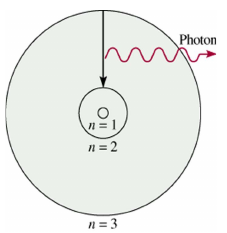
\includegraphics[width=5cm]{./imagenes/nivelesDeEnergia.png} \end{center}
        \begin{center} \textcolor{red}{\underline{Niveles de energía para el átomo de hidrógeno}} \end{center}
            \begin{center} 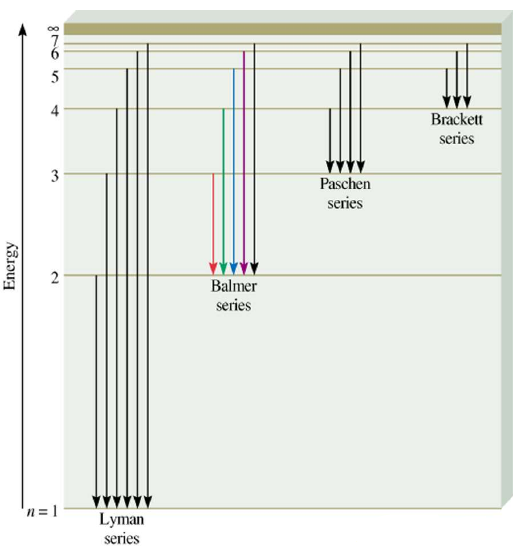
\includegraphics[width=6cm]{./imagenes/nivelesDeEnergia2.png} \end{center}

            \begin{center} 
                $E_{FOTON} = \Delta E = E_F - E_I$ \\[5pt]
                $E_F = - R_H (\frac{1}{{n_F}^{2}})$ \\[5pt]
                $E_I = -R_H (\frac{1}{{n_I}^{2}})$ \\[5pt]
                $\Delta E = R_H (\frac{1}{{n_I}^{2}} - \frac{1}{{n_F}^{2}}) = \hbar \times v$
            \end{center}


